\chapter{UAS Overview}\label{ch:uas}

In some cases it is necessary to talk about our system as a whole, such that we use it further. The Unmanned Aerial System (UAS) can be seen in Figure \ref{fig:uas} and it is composed of the following:
\begin{itemize}
	\item Drone
	\item Ground station (GS)
	\item Antennas
	\item DC Servomotor
\end{itemize}

\begin{figure}[H]
	\centering
	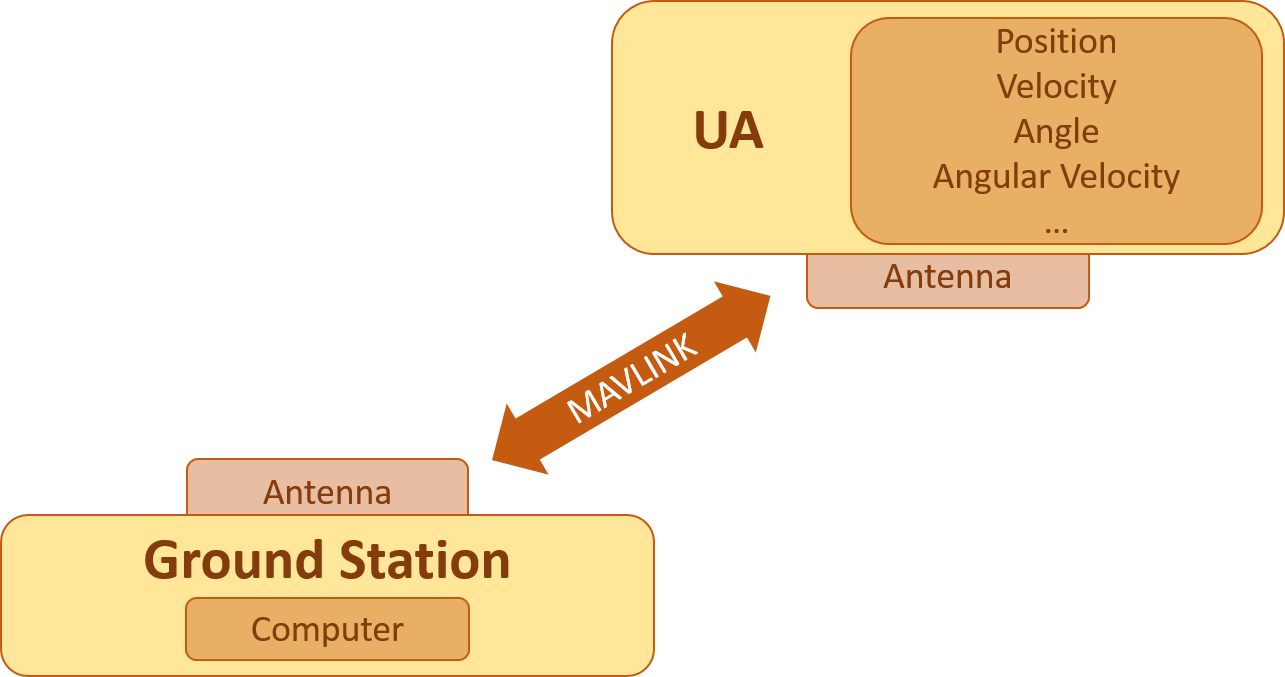
\includegraphics[scale=0.33]{figures/uas.png}
	\caption{Unmanned Aerial System Overview}
	\label{fig:uas}
\end{figure}

In order to have some bounds of the system we can have a look at the drone performances:
\begin{itemize}
	\item 50 km/h - stability at high speeds 
	\item 40 minutes - battery autonomy (30 minutes with payload)
	\item 2400 m - maximum flight altitude (higher if take off from mountain site)
	\item 50 km - maximum radio communication (with directional antennas)
	\item under 1 m - absolute positioning of X-Y GPS
	\item GPS return-to Home (automatically activates when radio link is lost)
\end{itemize}


